\begin{figure}[h]
    \centering
    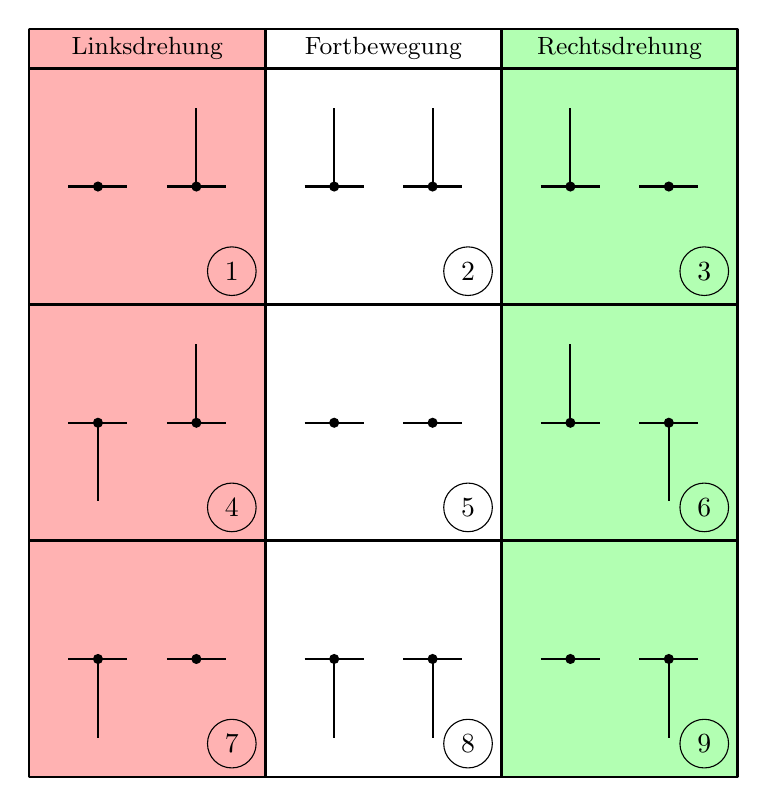
\begin{tikzpicture}[scale=0.5]
        \draw[line width=0.75, fill=red, opacity=0.3] (0,0) rectangle (6,19);
        \draw[line width=0.75, fill=green, opacity=0.3] (12,0) rectangle (18,19);

        \draw[line width=1] (0,0) -- (18,0);
        \draw[line width=1] (0,6) -- (18,6);
        \draw[line width=1] (0,12) -- (18,12);
        \draw[line width=1] (0,18) -- (18,18);
        \draw[line width=1] (0,0) -- (0,19);
        \draw[line width=1] (6,0) -- (6,19);
        \draw[line width=1] (12,0) -- (12,19);
        \draw[line width=1] (18,0) -- (18,19);
        \draw[line width=1] (0,19) -- (18,19);

        \node [anchor=center] at (3,18.5) {\small Linksdrehung};
        \node [anchor=center] at (9,18.5) {\small Fortbewegung};
        \node [anchor=center] at (15,18.5) {\small Rechtsdrehung};


        \draw[line width=0.75] (1,3) -- (2.5,3);
        \draw[line width=0.75] (3.5,3) -- (5,3);
        \draw[line width=0.75, fill=black] (1.75,3) circle (0.1);
        \draw[line width=0.75, fill=black] (4.25,3) circle (0.1);
        \draw[line width=0.75] (1.75,3) -- (1.75,1);
        \node[draw,circle] at (5.15,0.85) {7};

        \draw[line width=0.75] (7,3) -- (8.5,3);
        \draw[line width=0.75] (9.5,3) -- (11,3);
        \draw[line width=0.75, fill=black] (7.75,3) circle (0.1);
        \draw[line width=0.75, fill=black] (10.25,3) circle (0.1);
        \draw[line width=0.75] (7.75,3) -- (7.75,1);
        \draw[line width=0.75] (10.25,3) -- (10.25,1);
        \node[draw,circle] at (11.15,0.85) {8};

        \draw[line width=0.75] (13,3) -- (14.5,3);
        \draw[line width=0.75] (15.5,3) -- (17,3);
        \draw[line width=0.75, fill=black] (13.75,3) circle (0.1);
        \draw[line width=0.75, fill=black] (16.25,3) circle (0.1);
        \draw[line width=0.75] (16.25,3) -- (16.25,1);
        \node[draw,circle] at (17.15,0.85) {9};



        \draw[line width=0.75] (1,9) -- (2.5,9);
        \draw[line width=0.75] (3.5,9) -- (5,9);
        \draw[line width=0.75, fill=black] (1.75,9) circle (0.1);
        \draw[line width=0.75, fill=black] (4.25,9) circle (0.1);
        \draw[line width=0.75] (1.75,9) -- (1.75,7);
        \draw[line width=0.75] (4.25,9) -- (4.25,11);
        \node[draw,circle] at (5.15,6.85) {4};

        \draw[line width=0.75] (7,9) -- (8.5,9);
        \draw[line width=0.75] (9.5,9) -- (11,9);
        \draw[line width=0.75, fill=black] (7.75,9) circle (0.1);
        \draw[line width=0.75, fill=black] (10.25,9) circle (0.1);
        \node[draw,circle] at (11.15,6.85) {5};

        \draw[line width=0.75] (13,9) -- (14.5,9);
        \draw[line width=0.75] (15.5,9) -- (17,9);
        \draw[line width=0.75, fill=black] (13.75,9) circle (0.1);
        \draw[line width=0.75, fill=black] (16.25,9) circle (0.1);
        \draw[line width=0.75] (13.75,9) -- (13.75,11);
        \draw[line width=0.75] (16.25,9) -- (16.25,7);
        \node[draw,circle] at (17.15,6.85) {6};



        \draw[line width=0.75] (1,15) -- (2.5,15);
        \draw[line width=0.75] (3.5,15) -- (5,15);
        \draw[line width=0.75, fill=black] (1.75,15) circle (0.1);
        \draw[line width=0.75, fill=black] (4.25,15) circle (0.1);
        \draw[line width=0.75] (4.25,15) -- (4.25,17);
        \node[draw,circle] at (5.15,12.85) {1};

        \draw[line width=0.75] (7,15) -- (8.5,15);
        \draw[line width=0.75] (9.5,15) -- (11,15);
        \draw[line width=0.75, fill=black] (7.75,15) circle (0.1);
        \draw[line width=0.75, fill=black] (10.25,15) circle (0.1);
        \draw[line width=0.75] (7.75,15) -- (7.75,17);
        \draw[line width=0.75] (10.25,15) -- (10.25,17);
        \node[draw,circle] at (11.15,12.85) {2};

        \draw[line width=0.75] (13,15) -- (14.5,15);
        \draw[line width=0.75] (15.5,15) -- (17,15);
        \draw[line width=0.75, fill=black] (13.75,15) circle (0.1);
        \draw[line width=0.75, fill=black] (16.25,15) circle (0.1);
        \draw[line width=0.75] (13.75,15) -- (13.75,17);
        \node[draw,circle] at (17.15,12.85) {3};
    \end{tikzpicture}
    \caption{Die neun Bewegungszustände eines Rollstuhls}
    \label{fig:wheelstates}
\end{figure}